 \documentclass{beamer}

\usetheme{MagdeburgFIN}
\usefonttheme{structurebold}
\usepackage{graphicx}
\usepackage{wrapfig,lipsum}
\usepackage{float}
\usepackage{url}
\usepackage{pdfpages}
\usepackage[ngerman]{babel}
\usepackage[utf8]{inputenc}

\title{Thread Pool in GeckoDB/BOLSTER}
\subtitle{Milestone III: Implementation \& evaluation setup}
\author{Johann Wagner, Johannes Wünsche, Marten Wallewein-Eising, Robert Jenderise, Benedikt Zeilinger}
\date{\today}
\institute{Otto von Guericke University, Magdeburg}

\begin{document}

\begin{frame}[plain]
 \titlepage
\end{frame}

\section[Agenda]{}
	\begin{frame}
	\frametitle{Agenda}
	\tableofcontents
	\end{frame}

\section{Previously...}
\begin{frame}
	\begin{center}
		\huge Previously...
	\end{center}
\end{frame}

\begin{frame}
	\frametitle{Previously on Thread Pool in GeckoDB/BOLSTER}
	\begin{center}
		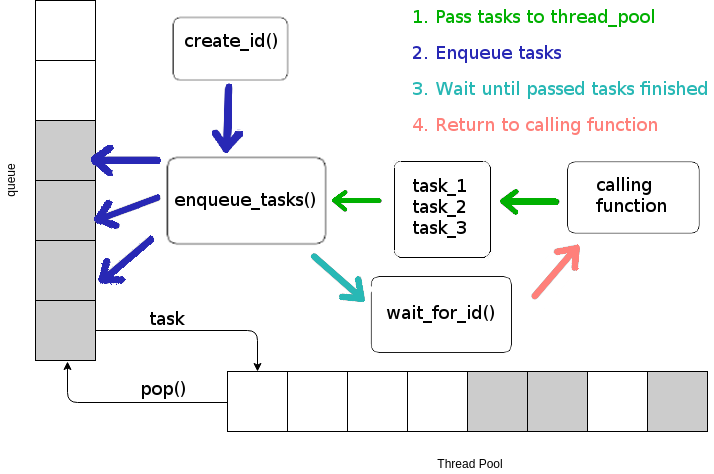
\includegraphics[width=0.9\textwidth]{img/pool_queue.png}
	\end{center}
\end{frame}

\begin{frame}
	\frametitle{Previously on Thread Pool in GeckoDB/BOLSTER}
	\begin{columns}
		\begin{column}{0.48\textwidth}
			\begin{itemize}
				\item Problem: waiting for a task to complete could lead to a
				race condition
				\item This was caused by the uncertainty of a thread\_task
				during transition between the priority queue and the
				thread pool
				\item Solution: slotmap with an atomic counter
			\end{itemize}
		\end{column}
		\begin{column}{0.48\textwidth}
			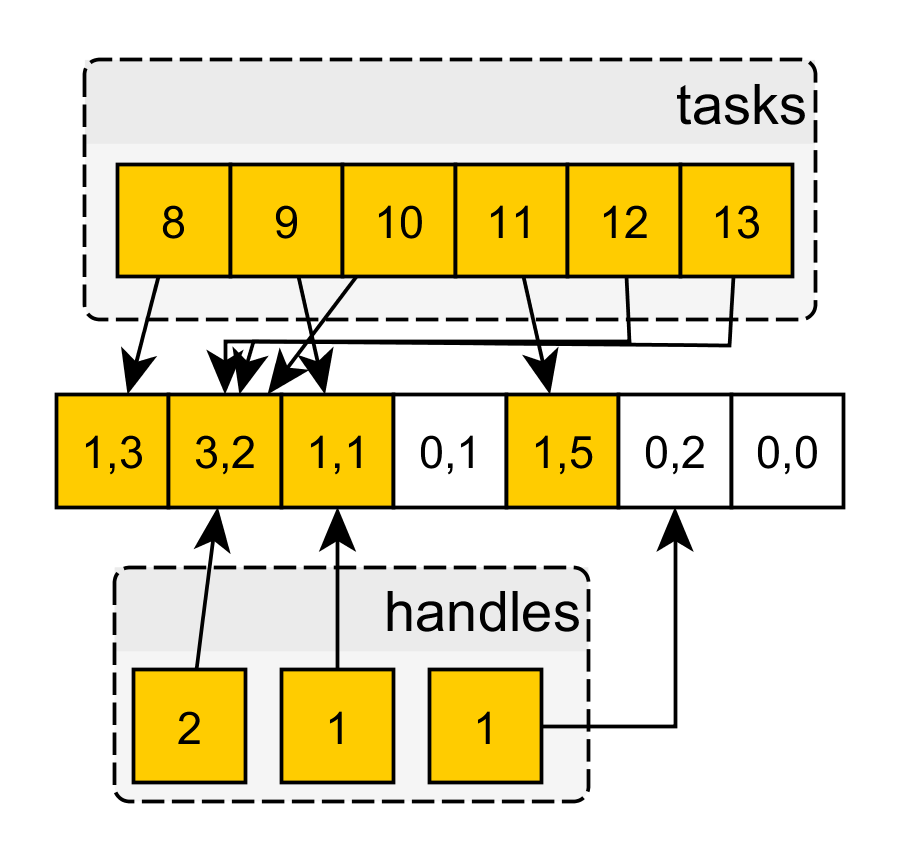
\includegraphics[width=1.0\textwidth]{waitingconcept.png}
		\end{column}
	\end{columns}
\end{frame}

\section{Implementation}
\begin{frame}
	\begin{center}
		\huge Implementation
	\end{center}
\end{frame}

\begin{frame}
	\frametitle{Design of Thread Pool System}
	\begin{center}
		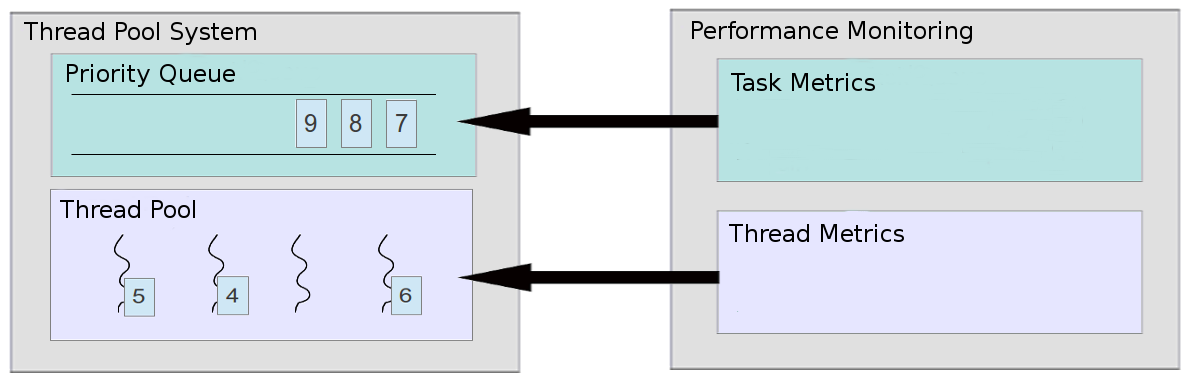
\includegraphics[width=0.9\textwidth]{img/pool_structure.png}
	\end{center}
	\begin{itemize}
		\item Thread pool system contains priority queue and thread pool itself
		\item Performance monitoring as optional, external component
	\end{itemize}
\end{frame}

\begin{frame}
	\frametitle{Implementation}
	We...
	\begin{itemize}
		\item Implemented task enqueueing and execution
		\item Implemented performance monitoring as external component
		\item Added gtest framework to project and wrote tests for pool and queue
		\item Started writing performance tests and measures for comparison against baseline ???
	\end{itemize}
\end{frame}

\begin{frame}
	\frametitle{Open issues}

\end{frame}

\section{Evaluation Setup}
\begin{frame}
	\begin{center}
		\huge Evaluation Setup
	\end{center}
\end{frame}

\begin{frame}
    \frametitle{Thank you for your attention!}
 	
\includegraphics[width=\textwidth]{img/important.jpg}
\end{frame}

\end{document}
